\chapter{メモリ割付け方式}
%プロセスが実行を開始する前に
物理メモリの一部をプロセスに割付け,
そこにプログラムをロードし実行する.
物理メモリを複数のプロセスで分割し利用するために,
幾つかの方式が考案されてきた.
ここでは,固定区画方式と可変区画方式について解説する.

%==============================================================================
\section{固定区画方式}

\begin{myfig}{btp}{固定区画方式}{fixedPartition}
  \begin{minipage}{0.49\columnwidth}
    \begin{center}
      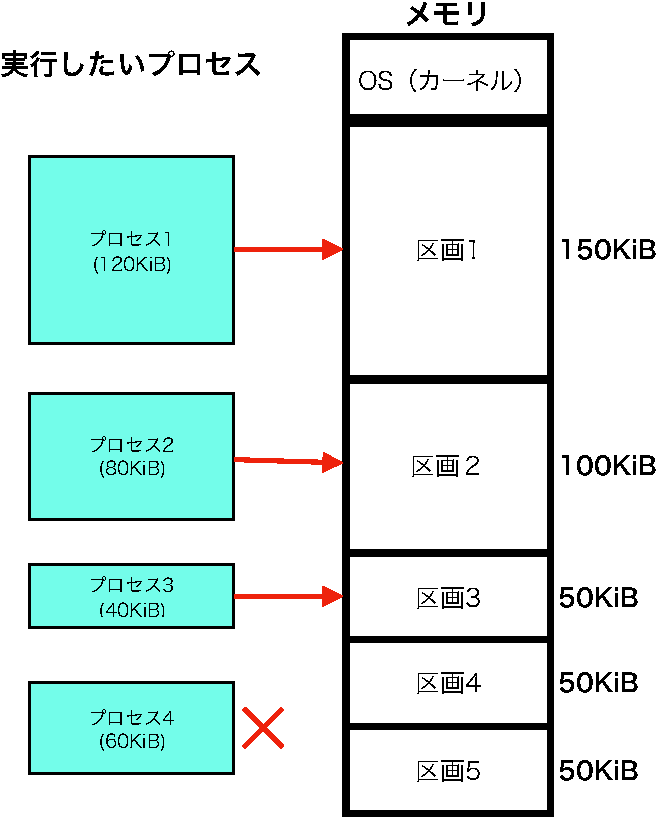
\includegraphics[scale=0.66]{Fig/fixedPartitionLoad-crop.pdf}
      \subcaption{区画を選択しプロセスをロード}
      \label{fig:fixedPartitionA}
    \end{center}
  \end{minipage}
  \begin{minipage}{0.49\columnwidth}
    \begin{center}
      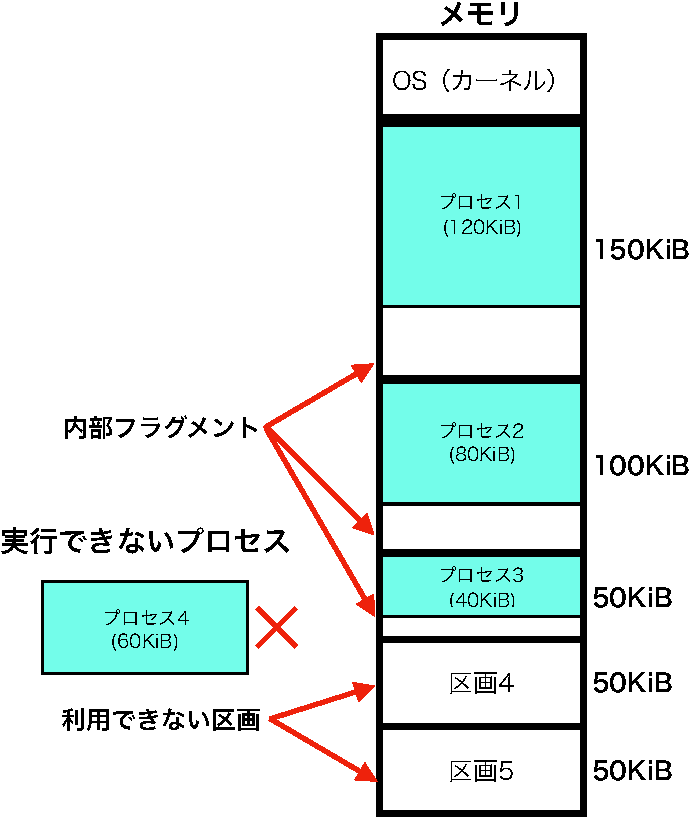
\includegraphics[scale=0.66]{Fig/fixedPartitionExec-crop.pdf}
      \subcaption{プロセスを実行}
      \label{fig:fixedPartitionB}
    \end{center}
  \end{minipage}
\end{myfig}

予めメモリを大小数種類の区画に分割しておく.
\figref{fixedPartition}の例では利用可能なメモリを五つの区画に分割している.
\figref{fixedPartitionA}はプロセス1から4を実行する場合を示している.
プロセスのサイズにより適切な区画を選択しプロセスをロードする.
プロセス4はロード可能な区画が無いので実行できない.

\figref{fixedPartitionB}の区画1から3ように,
区画の大きさとプロセスの大きさは一致するとは限らない.
内部に使用されない領域(\emph{内部フラグメント})が生じる.
また,区画4と区画5を合わせるとプロセス4をロード可能であるが,
固定区画方式では区画を組合せて利用することはできない.
仕組みは簡単だがメモリの利用率が低い.
特徴を以下にまとめる.

\begin{enumerate}
\item 空き領域の管理が容易である.
\item 領域内部に無駄な領域(\emph{内部フラグメント})が生じる.
\item 小さな領域が複数空いていても大きなプロセスは実行できない.
\item 実行可能なプロセスのサイズに強い制約がある.\\
  (図の例では,151KiBのプロセスは実行できない.)
\item 同時に実行できるプロセスの数に制約がある.\\
  (図の例では,同時に六つ以上のプロセスは実行できない.)
\end{enumerate}

%==============================================================================
\section{可変区画方式}
空き領域に必要に応じたサイズの区画を割付ける方式である.
\figref{variablePartition}に模式図を示す.

\begin{myfig}{btp}{可変区画方式}{variablePartition}
  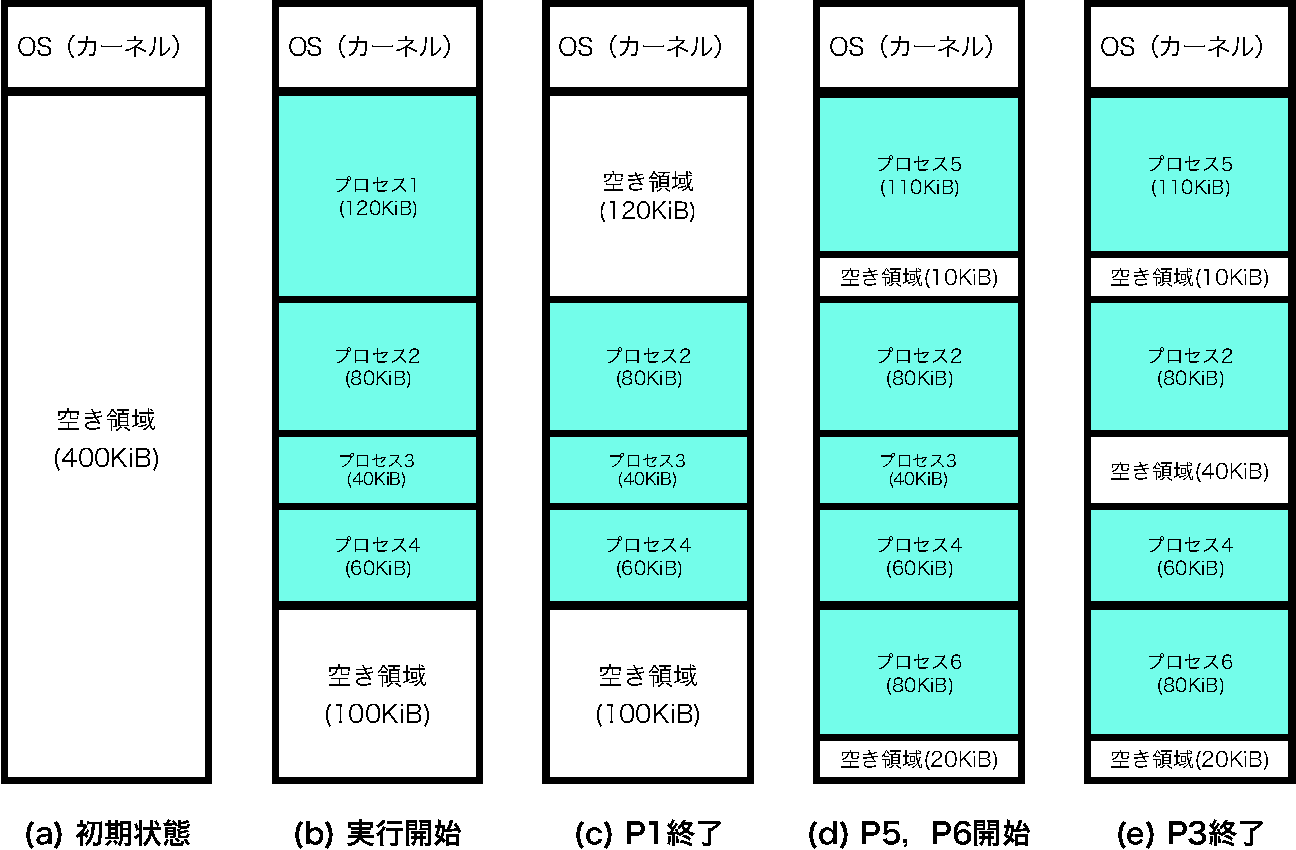
\includegraphics[scale=0.66]{Fig/variablePartition-crop.pdf}
\end{myfig}

\begin{enumerate}
\item[(a)] \emph{初期状態} \\
  メモリは,カーネル領域と一つの空き領域に分割される.
\item[(b)] \emph{実行開始} \\
  \figref{fixedPartition}と同じ四つのプロセスがロードされ実行を開始した.
  \figref{fixedPartition}の例では実行できなかった「プロセス4」も実行できる.
         (メモリの利用効率は良い.)
\item[(c)] \emph{プロセス1(P1)終了} \\
  終了したプロセスが利用していた領域は,
  再利用可能な空き領域になる.
\item[(d)] \emph{プロセス5(P5),プロセス6(P6)実行開始} \\
  120KiBの空き領域は,
  「110KiBの領域」と「10KiBの空き領域」に分割する.
  100KiBの空き領域は,
  「80KiBの領域」と「20KiBの空き領域」に分割する.
  プロセス5とプロセス6を新しい領域にロードし実行する.
\item[(e)] \emph{プロセス3(P3)終了} \\
  プロセス3が利用していた領域は,
  再利用可能な40KiB空き領域になる.
  メモリ全体では,10KiB,40KiB,20KiBの空き領域ができた.
\end{enumerate}

以上のように可変区画方式では,
プロセスの開始と終了が繰り返されるに従い小さな空き領域ができる.
このような区画の外にできる小さなメモリ領域を\emph{外部フラグメント}と呼ぶ.

%==============================================================================
\section{可変区画方式の空き領域選択方式}
以下の三つの方式が知られている.
\figref{firstBestWorstFit}に三つの方式で選択される空き領域の例を示す.

\begin{myfig}{btp}{空き領域の選択方式}{firstBestWorstFit}
  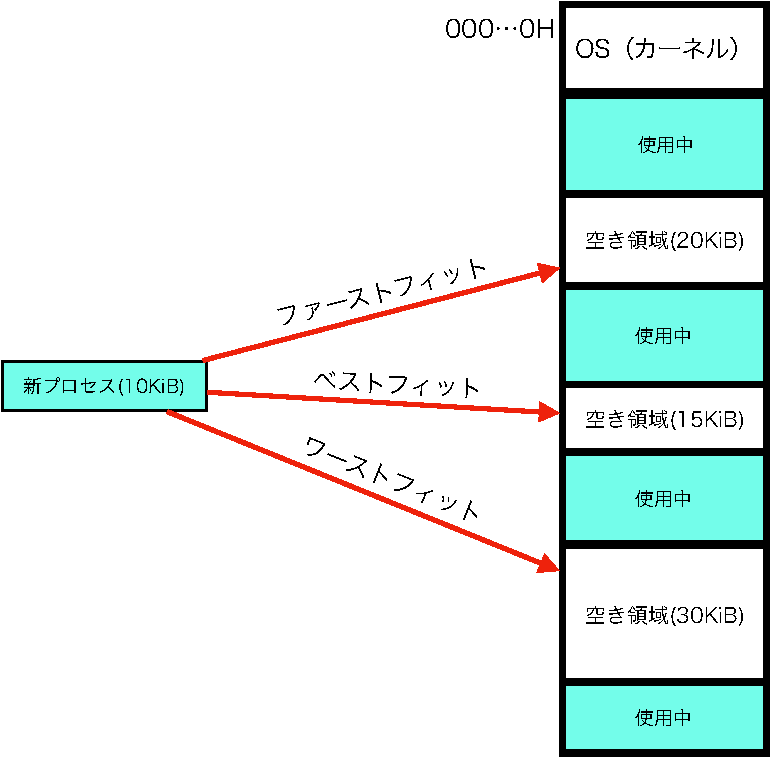
\includegraphics[scale=0.66]{Fig/firstBestWorstFit-crop.pdf}
\end{myfig}

\begin{itemize}
\item \emph{ファーストフィット(first-fit)方式}\\
  アドレス順に空き領域を探索し,
  最初に見つかった十分な大きさの領域を選択する.
\item \emph{ベストフィット(best-fit)方式}\\
  プロセスを格納可能な領域の中で最小のものを選択する.
\item \emph{ワーストフィット(worst-fit)方式}\\
  最も大きな領域を選択する.
\end{itemize}

シミュレーションの結果,
メモリ利用率の点でワーストフィット方式は最も性能が劣るが,
ファーストフィットとベストフィットの性能は互角だと言われている.
しかし実行時間の点で,
ファーストフィットがベストフィットより優れている\cite{MemoryAllocation}.

%==============================================================================
\section{空き領域の管理方式}
プロセスによって使用中のメモリ区画は,
プロセスのPCB等に記録しおけば見失う心配はない.
しかし,
どのプロセスにも属さない空き領域はメモリ管理側で記録しておく必要がある.

\begin{itemize}
\item \emph{ビットマップ(bitmap)方式}\\
  \figref{bitMap}のようにメモリを一定の大きさのブロックに分割し,
  1ブロックをビットマップの1ビットに対応させる.
  ビットが 0 ならブロックが空き状態,
  ビットが 1 なら使用中の意味になる.

  \begin{myfig}{btp}{ビットマップ方式}{bitMap}
    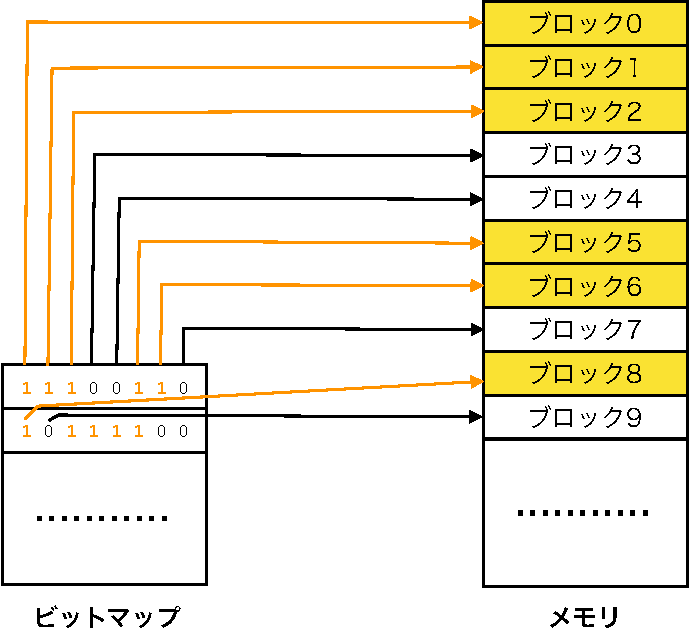
\includegraphics[scale=0.66]{Fig/bitMap-crop.pdf}
  \end{myfig}

  ビットマップはメモリ上に記録する.
  ビットマップの大きさは次のように計算できる.
  仮に8GiBのメモリを4KiBのブロックに分割して管理すると仮定すると,
  ブロックの総数は
  $8GiB \div 4KiB = (8\times 2^{30}) \div (4 \times 2^{10}) = 2 \times 2^{20}$
  個となる.
  ビットマップの大きさはブロック数と同じ$2 \times 2^{20}$ビットになる.
  これをバイト単位に換算すると,
  $(2 \times 2^{20}) \div 8 = 2^{18} = 256KiB$
  となる.

  ビットマップに使用するメモリは無視できるほど小さいものではない.
  ビットマップを小さくするにはブロックサイズを大きくすれば良い.
  しかし,ブロックサイズを大きくすると内部フラグメントが大きくなる.

\item \emph{リスト(linked-list)方式}\\
  空き領域をリストにして管理する方式である.
  使用中の領域が解放されると空き領域リストに追加される.
  解放される領域が,
  別の空き領域に隣接している場合は一つの空き領域になる.
  その様子を\figref{memFree}に示す.

  \begin{myfig}{btp}{領域開放時に空き領域を連結する様子}{memFree}
    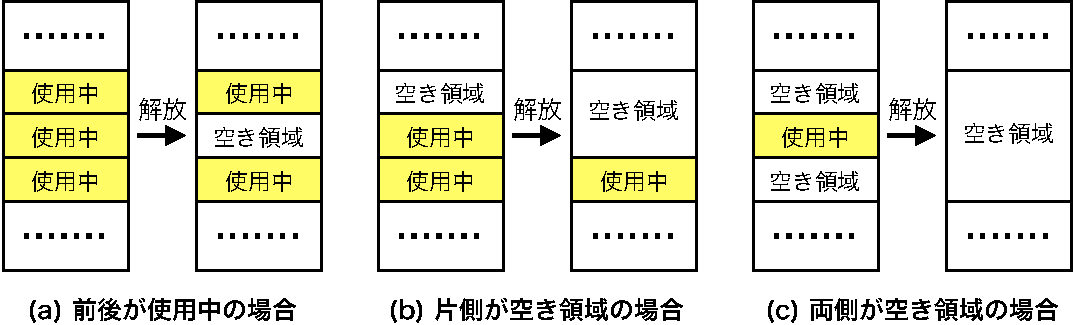
\includegraphics[scale=0.80]{Fig/memFree-crop.pdf}
  \end{myfig}

  リスト方式で用いるデータ構造の例を\figref{linkedList}に示す.
  新しい空き領域と前後の空き領域をマージする処理が簡単に行えるように,
  空き領域はアドレス順にソートしてリストに挿入される.

  \begin{myfig}{btp}{空き領域リスト}{linkedList}
    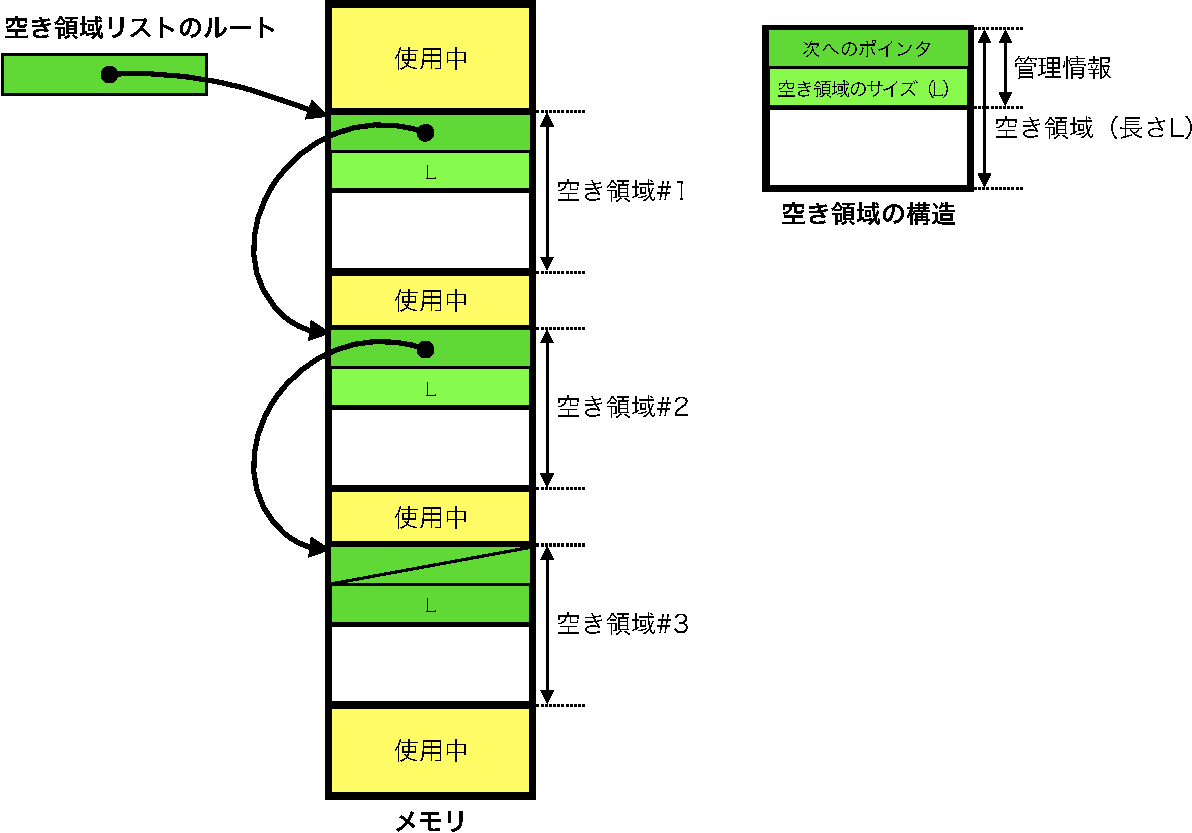
\includegraphics[scale=0.66]{Fig/linkedList-crop.pdf}
  \end{myfig}

  アドレス順に領域がソートしてあると,
  ファーストフィット方式で領域を探索するためにも適している.
  ベストフィット方式の場合は領域サイズ順にソートしてあると良いが,
  前述の空き領域のマージ処理には適さない.
\end{itemize}

%==============================================================================
\section{実装例}
第\ref{tacosMalloc}章にTacOSのメモリ割付けプログラムの例を示す.
この例は,可変区画方式,ファーストフィット方式のメモリ管理プログラムを
{\cmml}で実装したものである.

%==============================================================================
\section{まとめ}
物理メモリを分割しプロセスに割り付ける方式について学んだ.
予めメモリを分割しておく固定区画方式と,
必要に応じて分割する可変区画方式を紹介した.

可変区画方式における空き領域の選択方式には,
\emph{ファーストフィット方式},
\emph{ベストフィット方式},
\emph{ワーストフィット方式}があった.
また,空き領域の管理方式には,
\emph{ビットマップ方式},
\emph{リスト方式}があった.

%==============================================================================
\section*{練習問題}
\begin{enumerate}
  \renewcommand{\labelenumi}{\ttfamily\arabic{chapter}.\arabic{enumi}}
  \setlength{\leftskip}{1em}
\item 次の言葉の意味を説明しなさい.
  \begin{enumerate}
  \item 固定区画方式
  \item 可変区画方式
  \item 内部フラグメント
  \item 外部フラグメント
  \item ファーストフィット
  \item ベストフィット
  \item ワーストフィット
  \item ビットマップ方式
  \item リスト方式
  \end{enumerate}
\item 可変区画方式で管理される100KiBの空き領域がある時,
  次の順序で領域の割付け解放を行った.
  ファーストフィット方式を用いた場合と
  ベストフィット方式を用いた場合について,
  実行後のメモリマップを図示しなさい.
  \begin{enumerate}
  \item 30KiBの領域を割付け
  \item 40KiBの領域を割付け
  \item 20KiBの領域を割付け
  \item 先程割付けた40KiBの領域を解放
  \item 10KiBの領域を割付け
  \end{enumerate}
\item 本章ではカーネルがプロセスにメモリを割り付ける方式について学んだ.
  プロセスのアドレス空間では\|malloc()|関数がヒープセグメントに
  メモリを割り付ける.
  \|malloc()|関数の仕組みを調査しなさい.
\end{enumerate}
